\begin{center}
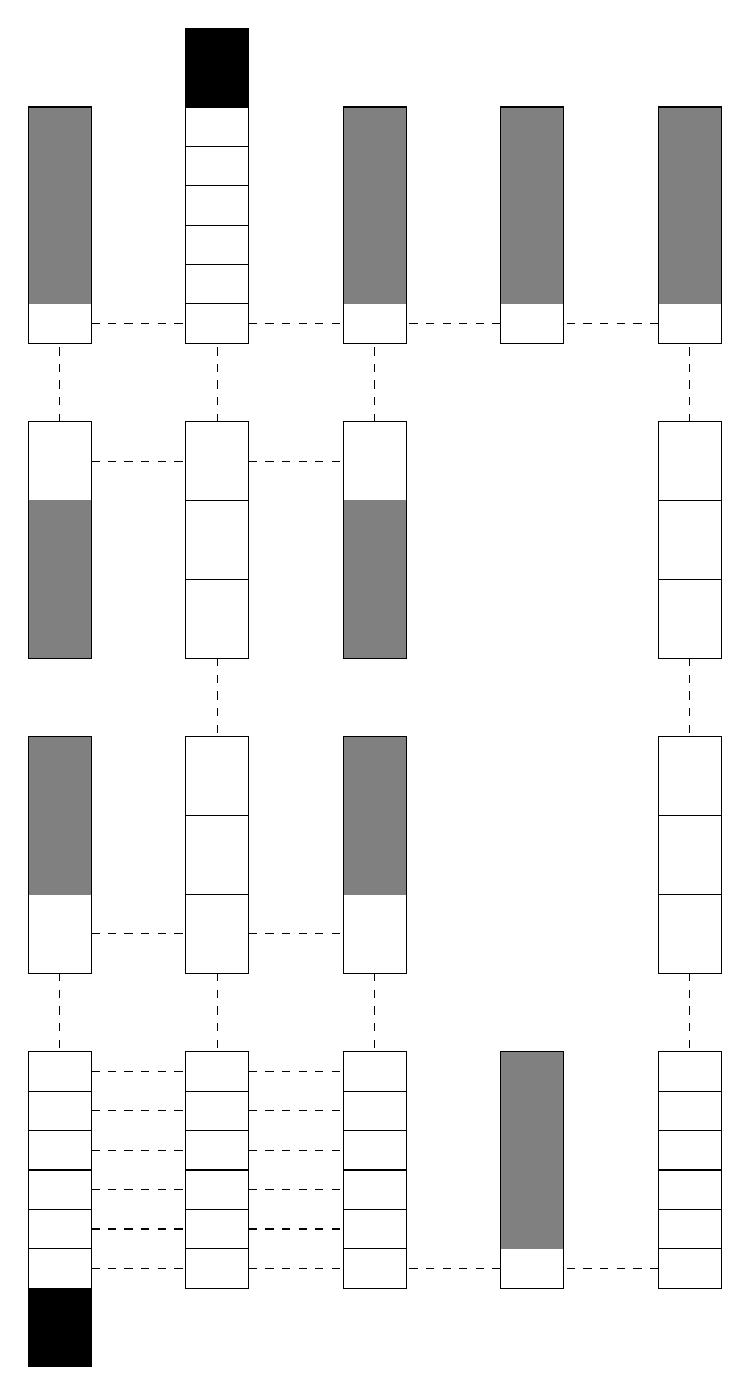
\begin{tikzpicture}
% \draw [thick] (-2,-3) rectangle (2,3);
% \draw [<->] (3.5,-3) -- (3.5,3);
% \draw (3.25,-3) -- (3.75,-3);
% \draw (3.25,3) -- (3.75,3);
% \draw [<->] (-2,-3.75) -- (2,-3.75);
% \draw (-2,-3.5) -- (-2,-4);
% \draw (2,-3.5) -- (2,-4);

% Middle rows of gray
\filldraw [gray] (-4.4,.5) rectangle (-3.6,2.5);
\filldraw [gray] (-.4,.5) rectangle (.4,2.5);
\filldraw [gray] (-4.4,-.5) rectangle (-3.6,-2.5);
\filldraw [gray] (-.4,-.5) rectangle (.4,-2.5);

% Top row of gray
\filldraw [gray] (-4.4,7.5) rectangle (-3.6,5);
\filldraw [gray] (-.4,7.5) rectangle (.4,5);
\filldraw [gray] (1.6,7.5) rectangle (2.4,5);
\filldraw [gray] (3.6,7.5) rectangle (4.4,5);

% Bottom row of gray
\filldraw [gray] (1.6,-7) rectangle (2.4,-4.5);

% Top and bottom row of rectangles
\foreach \x in {-4,-2,...,4}
\foreach \y in {-6,6}
{
\draw (\x,\y) +(-.4,-1.5) rectangle ++(.4,1.5);
}

% Middle rows of rectangles
\foreach \x in {-4,-2,0,4}
\foreach \y in {-2,2}
{
\draw (\x,\y) +(-.4,-1.5) rectangle ++(.4,1.5);
}

%Horizontal partitions
\foreach \y in {-7.5,-7,...,-4.5,-2.5,-1.5,1.5,2.5,4.5,5,...,7.5}
\draw (-1.6,\y) -- (-2.4,\y);

\foreach \y in {-7.5,-7,...,-4.5,-2.5,-1.5,1.5,2.5}
\draw (3.6,\y) -- (4.4,\y);

\foreach \y in {-7.5,-7,...,-4.5}
\draw (-3.6,\y) -- (-4.4,\y);

\foreach \y in {-7.5,-7,...,-4.5}
\draw (-.4,\y) -- (.4,\y);

% Vertical connections
\foreach \x in {-4,-2,0,4}
\draw [dashed] (\x,3.5) -- (\x,4.5);

\foreach \x in {-2,4}
\draw [dashed] (\x,.5) -- (\x,-.5);

\foreach \x in {-4,-2,0,4}
\draw [dashed] (\x,-3.5) -- (\x,-4.5);

% Black rectangles
\filldraw [black] (-1.6,7.5) rectangle (-2.4,8.5);

\filldraw [black] (-3.6,-7.5) rectangle (-4.4,-8.5);

%Horizontal connentions
\foreach \y in {4.75,3,-3,-4.75,-5.25,...,-7.25}
\draw [dashed] (-3.6,\y) -- (-2.4,\y);

\foreach \y in {4.75,3,-3,-4.75,-5.25,...,-7.25}
\draw [dashed] (-1.6,\y) -- (-.4,\y);

\foreach \y in {4.75,-7.25}
\draw [dashed] (1.6,\y) -- (.4,\y);

\foreach \y in {4.75,-7.25}
\draw [dashed] (3.6,\y) -- (2.4,\y);

\end{tikzpicture}
\end{center}
\label{fig:active_inactive}